
\documentclass[11pt, oneside]{article}   	% use "amsart" instead of "article" for AMSLaTeX format
\usepackage{geometry}                		% See geometry.pdf to learn the layout options. There are lots.
\geometry{letterpaper}                   		% ... or a4paper or a5paper or ... 
%\geometry{landscape}                		% Activate for for rotated page geometry
%\usepackage[parfill]{parskip}    		% Activate to begin paragraphs with an empty line rather than an indent
\usepackage{graphicx}				% Use pdf, png, jpg, or eps� with pdflatex; use eps in DVI mode
								% TeX will automatically convert eps --> pdf in pdflatex		
\usepackage{amssymb}

\title{Immanence}
\author{Paul Mathews, Timothy Barraclough}
\date{}							% Activate to display a given date or no date

\begin{document}
\maketitle
\section{Program Note}
%\subsection{}
Installation consisting of sonic and visual elements, designed to provide an unsettling experience through use of non-tactile sensors, reactive moving parts and live sampling of sound. Uses found objects to anchor a particular aesthetic with custom designed functional components. 
Conceptually functions to question issues of privacy as a fundamental civil liberty and the degradation of this ideal in a technological age. Provoked by the recent GCSB bill in New Zealand and the revelations concerning the NSA's wide ranging digital surveillance in the USA, this installation seeks to provoke observers to question their relationships with technology as a tool for the erosion of privacy by using simple and easily obtainable data to produce an awkward technological response.
The mechanical components are three motors which react to proximity of nearby people. The sonic component is the results of the motors motion and the live sampling. The live sampling is enabled by a spatial threshold and triggered through analysis of the incoming signal, hoping to capture a viewer's reaction. The recorded sound is processed by producing a random population of playback units of different sizes and rates and running an evolutionary simulation upon the population, causing it to procedurally morph towards a target parameter vector which is chosen for unsettling effect and situated to the space using environmental data.


\section{Audio Example}

An audio example can be found at this URL : \\

https://soundcloud.com/pfcmathews/immanence-example\\
\\
\\
\\
\\
\\

\section{Illustration}
\begin{figure}[htl]
\centering
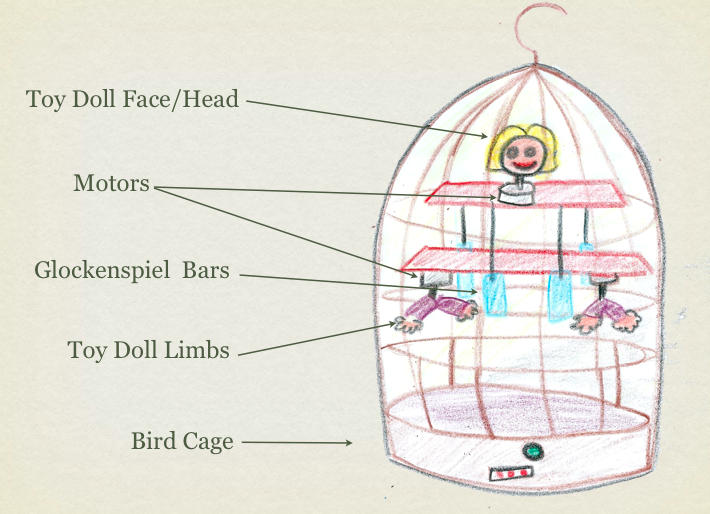
\includegraphics[width=150mm]{Diagram.png}

\end{figure}



\end{document}  